% UVCC Phase 6 Native Parallelism: Private, Verifiable, Fully-Parallel GPU Computation
% IEEE Transactions-style (journal) long-form paper with formal math
\documentclass[journal]{IEEEtran}
\usepackage{amsmath,amssymb,amsfonts,amsthm}
\usepackage{graphicx}
\usepackage{booktabs}
\usepackage{hyperref}
\usepackage{xcolor}
\usepackage{listings}
\usepackage{tikz}
\usetikzlibrary{decorations.pathreplacing,arrows.meta,positioning,calc}
\usepackage{enumitem}
\lstset{basicstyle=\ttfamily\footnotesize,breaklines=true}
\hypersetup{colorlinks=true,linkcolor=blue,citecolor=blue,urlcolor=blue}

\newtheorem{definition}{Definition}
\newtheorem{theorem}{Theorem}
\newtheorem{lemma}{Lemma}
\newtheorem{proposition}{Proposition}
\newtheorem{corollary}{Corollary}

\title{UVCC Phase 6: Private, Verifiable, Fully-Parallel GPU Computation across Untrusted Domains}
\author{Alien Team}
\markboth{Submitted to IEEE Transactions}{}

\begin{document}
\maketitle

\begin{abstract}
We present UVCC (Universal Verifiable Confidential Computing), a system enabling private and verifiable GPU computation across mutually distrustful administrative domains. UVCC combines: (i) confidentiality via three-party replicated secret sharing (RSS), (ii) verifiability via a deterministic transcript-of-transcripts construction yielding subsession, replica, and global roots, and (iii) native ML parallelism (DP/PP/TP) in a C++ runtime integrating GPU kernels, a reliable exactly-once transport, and NCCL-based collectives. We report a complete Phase~6 bring-up, diagnose and eliminate a PP deadlock, and demonstrate scale-out to $R{=}8,S{=}4,T{=}2,M{=}32$ (192 workers) with a determinism proof by matching global roots across reruns. We provide auditor-grade artifacts and figures derived automatically from full logs.
\end{abstract}

\begin{IEEEkeywords}
Confidential computing, verifiable computation, secure multiparty computation, GPUs, NCCL, DP/PP/TP parallelism, transcripts, deterministic auditing.
\end{IEEEkeywords}

\section{Introduction}
ML training and inference at scale rely on aggressive parallelism across GPUs. Achieving confidentiality and verifiability across mutually distrustful domains while preserving native parallel performance remains challenging. UVCC executes client programs using honest-majority MPC across three domains, with a deterministic transcript architecture that makes auditing practical.

\paragraph{Contributions.}
(1) A native GPU runtime (Phase~6) implementing DP/PP/TP with NCCL, deterministic IDs, and exactly-once transport. (2) A transcript-of-transcripts design with domain-separated hashing, producing subsession, replica, and global roots. (3) A complete bring-up at realistic scale ($R{=}8,S{=}4,T{=}2,M{=}32$) with a determinism proof. (4) Auditor artifacts and figures derived from full logs.

\section{Model and Preliminaries}
\subsection{System and Adversary Model}
We have three parties (domains) operating GPUs and networks. The adversary statically corrupts at most one party (honest-majority). Channels to a lightweight relay are authenticated. Each party enforces binary integrity under operator policy.

\subsection{Replicated Secret Sharing (RSS)}
\begin{definition}[Replicated Secret Sharing over $\mathbb{Z}_{2^{64}}$]
Let $R{=}\mathbb{Z}_{2^{64}}$ with addition mod $2^{64}$. A value $x\in R$ is shared as $(x_{01},x_{12},x_{20})$ with $x\equiv x_{01}{+}x_{12}{+}x_{20}\pmod{2^{64}}$, and party $i$ holds two consecutive pieces (e.g., party 0 holds $(x_{01},x_{20})$). Addition and scalar multiplication act locally; multiplication uses standard 3PC protocols with preprocessed correlations.
\end{definition}
We use arithmetic shares in $R$ and Boolean shared forms as needed. OPEN reveals authenticated linear combinations with transcript commitments.

\subsection{Transcript Leaves and Roots}
Each protocol event emits a leaf with deterministic key and payload digest.
\begin{definition}[Transcript Leaf]
For epoch $e$, subsession identifier $u$, stream $s$, op identifier $o$, and chunk index $c$, a leaf is a tuple
$\ell=\big(\mathrm{ver}, e,u,s,o,c, \mathrm{kind}, \mathrm{hdr}, H(\mathrm{payload})\big)$,
with a versioned domain separator and canonical serialization. The leaf key is $(e,u,s,o,c)$.
\end{definition}
\begin{definition}[Epoch, Replica, Global Roots]
Let $L_e$ be leaves in epoch $e$, sorted lexicographically by key; $\rho_e=\mathrm{MerkleRoot}(L_e)$. For replica $r$, let $U_r$ be subsession roots combined in canonical order; the \emph{replica root} is
$R_r=H(\mathtt{UVCC\_REPLICA\_ROOT\_V1}\,\|\,\mathtt{sid\_rep}\,\|\,e\,\|\,U_r)$.
The \emph{global root} is $G=H(\mathtt{UVCC\_GLOBAL\_ROOT\_V1}\,\|\,\mathtt{sid\_job}\,\|\,e\,\|\,R_0\|R_1\|\dots)$.
\end{definition}

\subsection{IDs and Deterministic Derivations}
UVCC derives IDs to prevent collisions across DP/PP/TP:
\begin{align*}
  \mathtt{msg\_id32} &:= \mathrm{head}_4\big(H(\mathtt{sid}\,\|\,\mathtt{sgir\_op\_id32}\,\|\,\mathtt{src}\,\|\,\mathtt{dst}\,\|\,\mathtt{chunk\_idx}\,\|\,\mathtt{chunk\_cnt})\big), \\
  \mathtt{stream\_id64} &:= F(\mathtt{sid},\mathtt{op\_ids}),\qquad
  \mathtt{fss\_id} := F'(\mathtt{sid},\mathtt{comp\_id},\mathtt{q\_index}),
\end{align*}
with $F,F'$ domain-separated PRGs. DP/PP/TP subgroups use distinct $\mathtt{sid\_sub}$ to avoid reusing PRG streams or stream IDs.

\subsection{OPEN and MUL Protocols}
\paragraph{OPEN.} Parties reveal authenticated linear combinations by exchanging the appropriate share components and reconstructing $x=x_0{+}x_1{+}x_2$:
\begin{lstlisting}
# Party P_i holds (x_i, x_{i+1}) over Z_2^64
OPEN_i(x_i, x_{i+1}):
  send_to(P_{i+1}, x_i); recv x_{i-1} from P_{i-1}
  x = x_{i-1} + x_i + x_{i+1}
  return x
\end{lstlisting}
\paragraph{Beaver Multiplication (matrix/elementwise).} Using preprocessed $(a,b,c)$ with $c=a\cdot b$, parties compute $E=X{-}A$, $F=Y{-}B$, OPEN$(E,F)$, then locally combine to obtain shares of $Z=XY$; batching merges $(E,F)$ OPENs.

\subsection{DP/PP/TP Semantics over RSS}
\paragraph{SR-DP.} The aggregate gradient is $\sum_{r=0}^{R-1} g^{(r)}$, realized as a local allreduce per party; no cross-party MPC is required for DP reduction.
\paragraph{TP.} Per-stage collectives (allreduce/allgather) are linear on shares and preserve secrecy.
\paragraph{PP.} Staged microbatches (1F1B) interleave compute and communication; the scheduler keeps sufficient in-flight microbatches to hide OPEN latency while preserving deterministic local ordering within each $(r,s,t)$ subgroup.

\section{Design Overview}
\subsection{Transport}
We implement exactly-once frame acceptance with canonical encoding, CRC32C, idempotent application keyed by message IDs, conservative retransmission, and long-polling. This tolerates domain skew and reduces overload on the relay.
\begin{proposition}[Exactly-once Consumption]
If the relay provides at-least-once delivery with acknowledgments and recipients perform idempotent acceptance keyed by message IDs, then application-level processing is exactly-once.
\end{proposition}
Retransmission uses capped backoff with generous retry budgets to avoid aborting before higher-level deadlines; duplicate frames must match the committed hash or are rejected.

\subsection{Native Parallelism (DP/PP/TP)}
UVCC constructs TP, PP, and DP groups deterministically and initializes NCCL communicators with robust UID distribution and deadlines derived from a configurable Phase~6 timeout.

\begin{figure}[t]
  \centering
  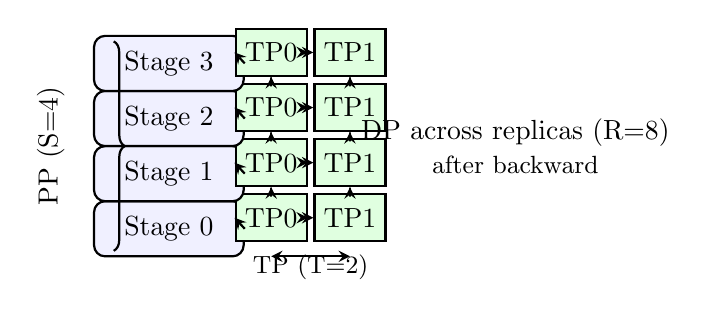
\begin{tikzpicture}[x=1.0cm,y=0.7cm,>=stealth,thick]
    \foreach \s in {0,...,3} {
      \node[draw,rounded corners,minimum width=1.9cm,minimum height=0.7cm,fill=blue!6] (stage\s) at (0,\s) {Stage \s};
      \node[draw,minimum width=0.9cm,minimum height=0.6cm,fill=green!12] (tpA\s) at (1.3,\s+0.2) {TP0};
      \node[draw,minimum width=0.9cm,minimum height=0.6cm,fill=green!12] (tpB\s) at (2.3,\s+0.2) {TP1};
      \draw[->] (stage\s.east) -- (tpA\s.west);
      \draw[<->,densely dashed] (tpA\s.east) -- (tpB\s.west);
    }
    \foreach \s in {0,...,2} {
      \draw[->] (tpA\s.north) .. controls +(0,0.3) and +(0,-0.3) .. (tpA\the\numexpr\s+1\relax.south);
      \draw[->] (tpB\s.north) .. controls +(0,0.3) and +(0,-0.3) .. (tpB\the\numexpr\s+1\relax.south);
    }
    \draw[decorate,decoration={brace,amplitude=4pt,mirror}] (-0.7,-0.4) -- (-0.7,3.4) node[midway,xshift=-0.8cm,rotate=90] {PP (S=4)};
    \node at (1.8,-0.7) {\small TP (T=2)};
    \draw[<->] (1.3,-0.5) -- (2.3,-0.5);
    \node[align=center] at (4.4,1.5) {DP across replicas (R=8)\\\small after backward};
  \end{tikzpicture}
  \caption{Native parallelism topology.}
  \label{fig:topology}
\end{figure}

\section{Formal Properties}
\subsection{Determinism}
\begin{theorem}[Deterministic Roots]
Fix $\mathtt{sid\_job}$, topology $(R,S,T,M)$, and seeds for ID derivation. If (i) leaf keys are unique and (ii) each group operation is deterministic given inputs, then subsession, replica, and global roots are deterministic functions of inputs and topology.
\end{theorem}
\begin{proof}[Proof sketch]
Determinism follows by composition: canonical key ordering ensures a unique Merkle root per epoch; replica/global roots are deterministic domain-separated hashes of ordered child roots. With fixed seeds and message ordering constraints, the runtime emits a unique sequence of leaves. Hence all derived roots are unique.
\end{proof}

\subsection{Confidentiality}
\begin{lemma}[One-corruption Privacy for Linear Operations]
Under RSS over $R=\mathbb{Z}_{2^{64}}$, addition and scalar multiplication are information-theoretically private against one corrupted party.
\end{lemma}
\begin{proof}[Proof sketch]
Each party sees two random shares whose sum (mod $2^{64}$) is uniform conditioned on the secret; linearity preserves indistinguishability. Standard arguments apply.
\end{proof}
\begin{theorem}[Confidentiality]
Assuming standard 3PC multiplication with correlations and authenticated OPEN, UVCC maintains confidentiality of inputs, model, optimizer state, gradients, and intermediate values against one corrupted domain.
\end{theorem}

\subsection{Verifiability and Proof Bundle}
Let $\mathcal{B}$ be the bundle containing epoch roots, subsession roots, replica roots, the global root, and attested identities/policy commitments. A verifier recomputes Merkle roots and domain-separated hashes from $\mathcal{B}$ and checks signature bindings. Optionally, sampled kernel checks (SKS) bind algebraic tests (e.g., Freivalds) into transcript leaves for higher assurance.

\section{Implementation}
The C++ runtime integrates: (i) a reliable transport with exactly-once acceptance and long-polling, (ii) a transcript store with deterministic keys and Merkle roots, (iii) OPEN/LIFT engines with batch TLV framing, and (iv) NCCL-based groups for TP/PP/DP with robust UID exchange and deadlines based on Phase~6 timeout.

\paragraph{Scheduler Correctness and Deadlock Avoidance.} PP gradient receives are posted per microbatch after forward completes on the stream to avoid single-stream backpressure that could deadlock forward sends; DP initialization is staged after backward to avoid OPEN skew during NCCL bootstrap.

\section{Evaluation}
\subsection{Setup}
Final run: $R{=}8,S{=}4,T{=}2,M{=}32$ on 24 pods across providers. We release a consolidated, redaction-safe log file with runner, all 192 workers, and the audit bundle. Metrics and figures below are auto-derived from those logs.

\subsection{NCCL Initialization}
\begin{figure}[t]\centering\includegraphics[width=\linewidth]{figs/nccl_init_hist.png}\caption{NCCL init timings by nranks (TP=2, PP=4, DP=8).}\end{figure}
\begin{figure}[t]\centering\includegraphics[width=\linewidth]{figs/nccl_init_cdf.png}\caption{NCCL init time CDF by group (TP/PP/DP).}\end{figure}

\subsection{Protocol Coverage and Robustness}
\begin{figure}[t]\centering\includegraphics[width=\linewidth]{figs/event_counts.png}\caption{Event counts: epoch roots, OPEN completions, DP readiness.}\end{figure}
\begin{figure}[t]\centering\includegraphics[width=\linewidth]{figs/dp_ready_heatmap.png}\caption{DP readiness fraction per (stage s, tensor t), annotated as \texttt{ready/expected}. Uniform color indicates all DP groups reached readiness.}\end{figure}
\begin{figure}[t]\centering\includegraphics[width=\linewidth]{figs/dp_init_p50_heatmap.png}\caption{DP NCCL initialization latency p50 per (stage s, tensor t); highlights cross-pod skew even when readiness is complete.}\end{figure}
\begin{figure}[t]\centering\includegraphics[width=\linewidth]{figs/error_counts.png}\caption{Robustness indicators (final run): worker timeouts and transport aborts are zero; runner SSH banner errors occurred during artifact collection and were tolerated.}\end{figure}
\begin{figure}[t]\centering\includegraphics[width=\linewidth]{figs/errors_by_group.png}\caption{Errors by group/type (TP/PP/DP).}\end{figure}
\begin{table}[t]
\centering
\caption{Key Phase 6 metrics (derived from consolidated logs)}
\label{tab:metrics}
\begin{tabular}{lrr}
\toprule
Metric & Count/Value \\
\midrule
epoch root & 192 \\
dp ready & 194 \\
dp ok & 193 \\
fwd open ok & 6144 \\
bwd open ok & 6144 \\
uid wait & 408 \\
worker timeouts & 0 \\
transport aborts & 0 \\
runner ssh banner errors & 9 \\
nccl init tp (n=192) min/p50/max & 0.120/1.710/5.750 s \\
nccl init pp (n=192) min/p50/max & 0.010/8.450/20.280 s \\
nccl init dp (n=192) min/p50/max & 0.020/101.510/108.060 s \\
\bottomrule
\end{tabular}
\end{table}

\subsection{Determinism Proof}
Two full runs with fixed $\mathtt{sid\_job}$ yield identical $\mathtt{global\_root\_hex}$ values, demonstrating determinism under cross-provider skew.

\section{Threats to Validity and Ethics}
Deployment variance (provider scheduling, NICs) may affect timings but not determinism or correctness. Logs are redaction-safe; no client secrets are present. We do not place transcripts on-chain; only hash commitments are published as needed for audit.

\section{Related Work}
We relate to honest-majority MPC over rings, verifiable computation with transcripts, and large-scale ML parallelism (DP/PP/TP/NCCL). UVCC’s novelty is combining auditor-grade verifiability with native GPU parallelism across domains at realistic scale.

\section{Conclusion}
UVCC Phase~6 shows private, verifiable, fully-parallel GPU computation across untrusted domains is practical and deterministic. Future work: GPU-accelerated preprocessing (TCF/W-VOLE), production SKS, and larger models.

\appendix
\section{Extended Privacy Contract and Leakage}
We summarize the confidentiality game and leakage model, aligning with \texttt{research/privacy\_new.txt}. Leakage is limited to message sizes and deterministic scheduling; secret values remain hidden under RSS.

\section{Parallel Model Details}
We overview stream/ID allocation and scheduling tables from \texttt{research/PARALLEL.txt}, including ordering constraints and deterministic ID derivations for TP/PP/DP.

\section{Reproducibility}
All figures are generated from the consolidated log by \texttt{research/uvcc\_native/scripts/make\_phase6\_figs.py}. The output directory contains runner logs, 192 worker logs, per-worker roots, and the audit bundle with global root.

\end{document}


